\section{Budowa robota}

\textbf{Główna konstrukcja} \newline
Robot został zbudowany w oparciu o konstrukcję lasera CNC małej mocy. Główna rama, po której porusza się mocowanie z kamerą, zbudowana jest z profili aluminiowych skręconych śrubami.
Urządzenie posiada dwie sterowalne osie napędzane przy pomocy pasków maszynowych i silników krokowych. 
Konstrukcja stoi na aluminiowych nogach przymocowanych do ramy poprzez wydrukowane na drukarce 3D tuleje zaciskowe. 
Rozwiązanie to pozwala na regulację każdej nogi osobno i ustawienie poziomu. 
\begin{figure}[H]
	\centering
	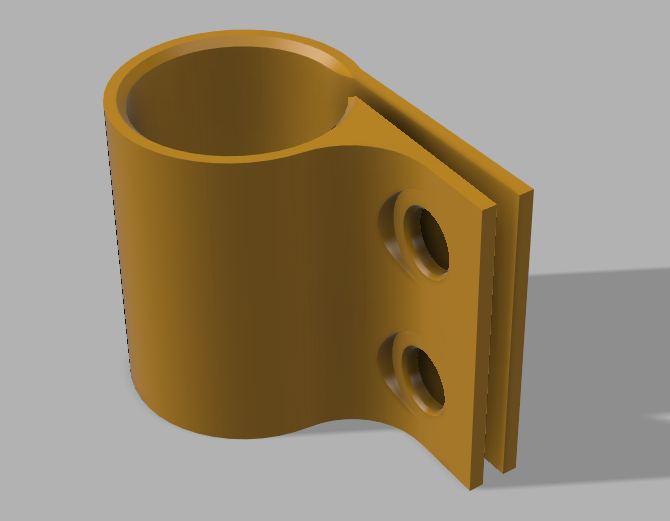
\includegraphics[height=4.5cm]{pages/dodatekARobot/img/model3DMocowaniaNog.png}
    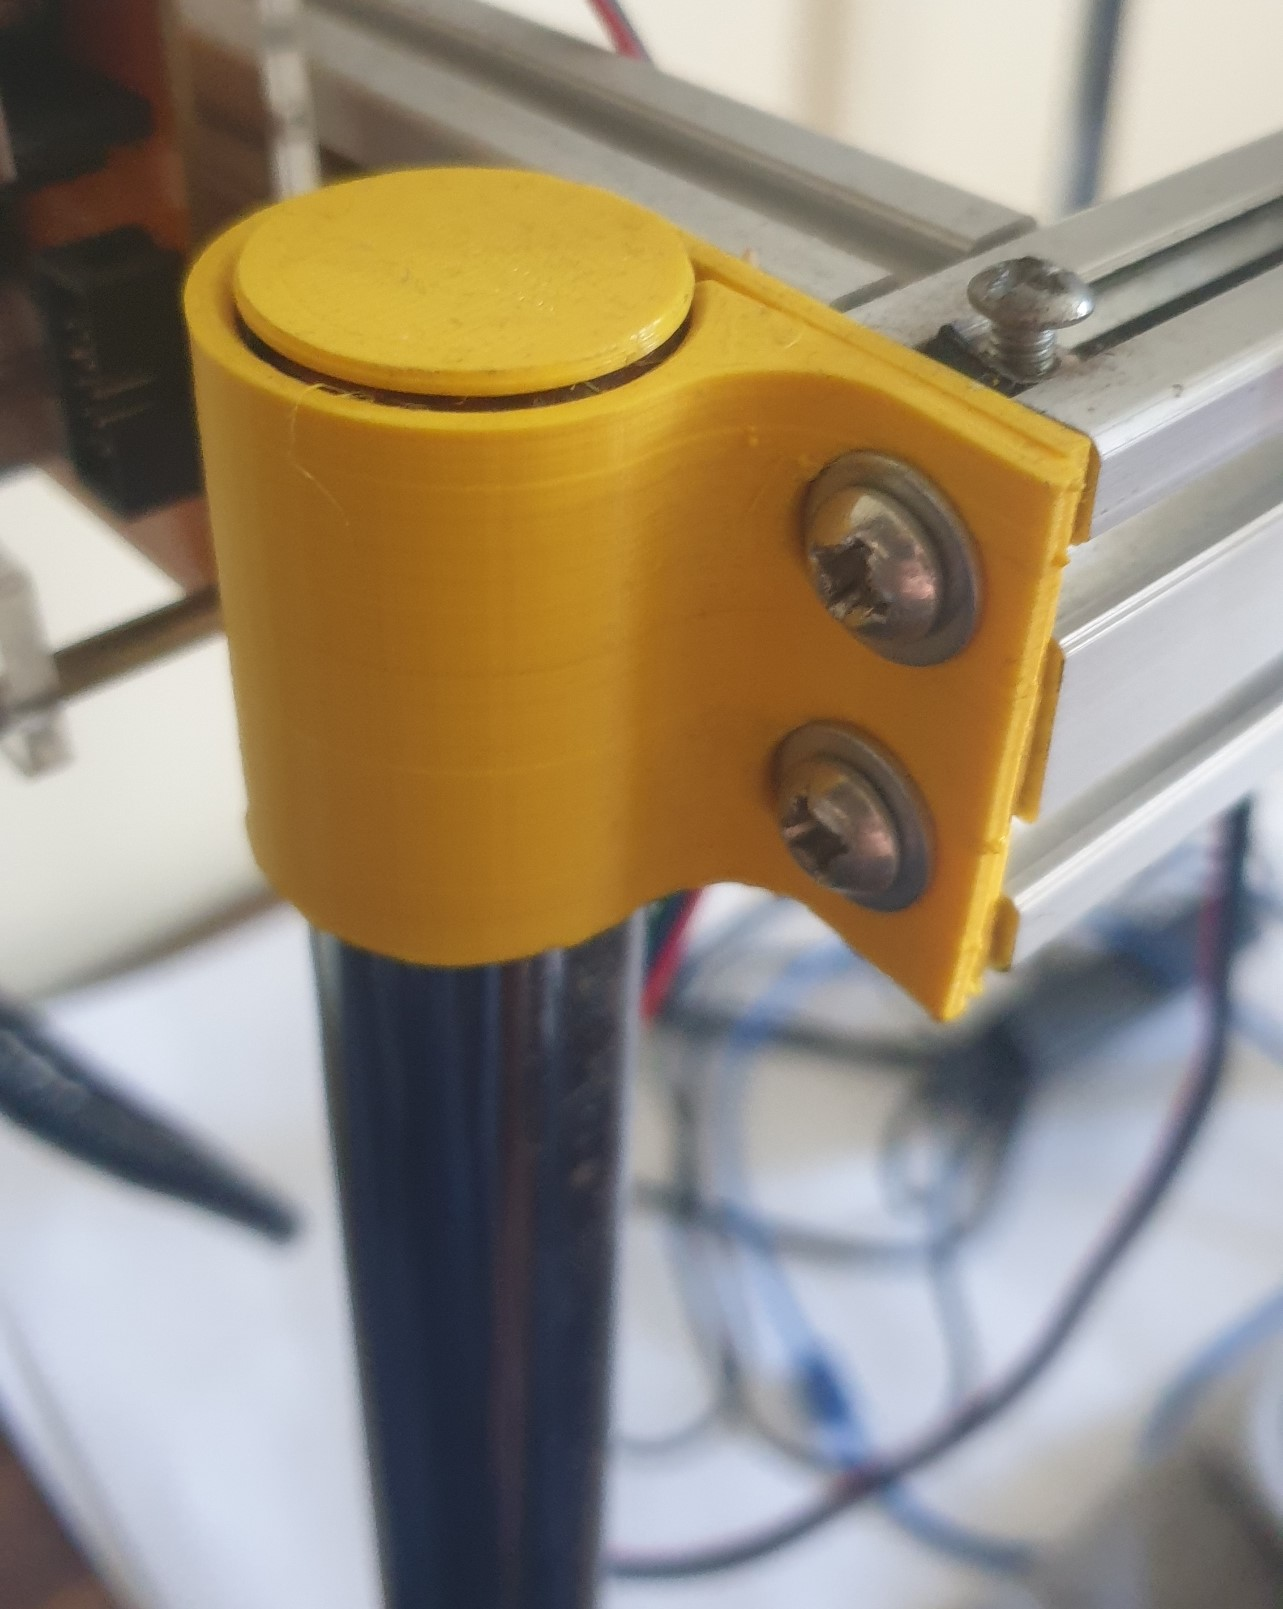
\includegraphics[height=4.5cm]{pages/dodatekARobot/img/mocowanieNogi.jpg}
	\caption{Mocowanie nóg robota, model i zdjęcie z robota}
	\label{rys:model3DMocowanieNog}
\end{figure}
Wszystkie opisywane dalej modele zostały wydrukowane z materiału 'PLA' w temperaturze ok. 210$^\circ$C i wysokością warstwy 0,15mm.

\textbf{Mocowanie kamery} \newline
Moduł z laserem został zdemontowany, a do oryginalnego uchwytu zaprojektowane zostało mocowanie telefonu, będącego w tym przypadku kamerą. 
\begin{figure}[H]
	\centering
	\begin{subfigure}{}
		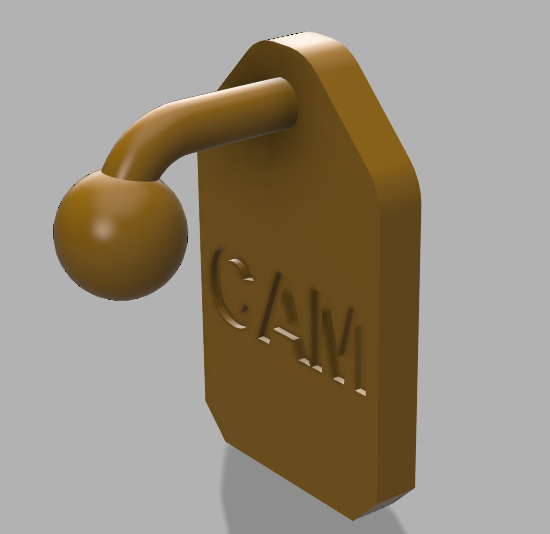
\includegraphics[height=4.5cm]{pages/dodatekARobot/img/model3DMocowaniaKamery.png}
	\end{subfigure}
	\begin{subfigure}{}
		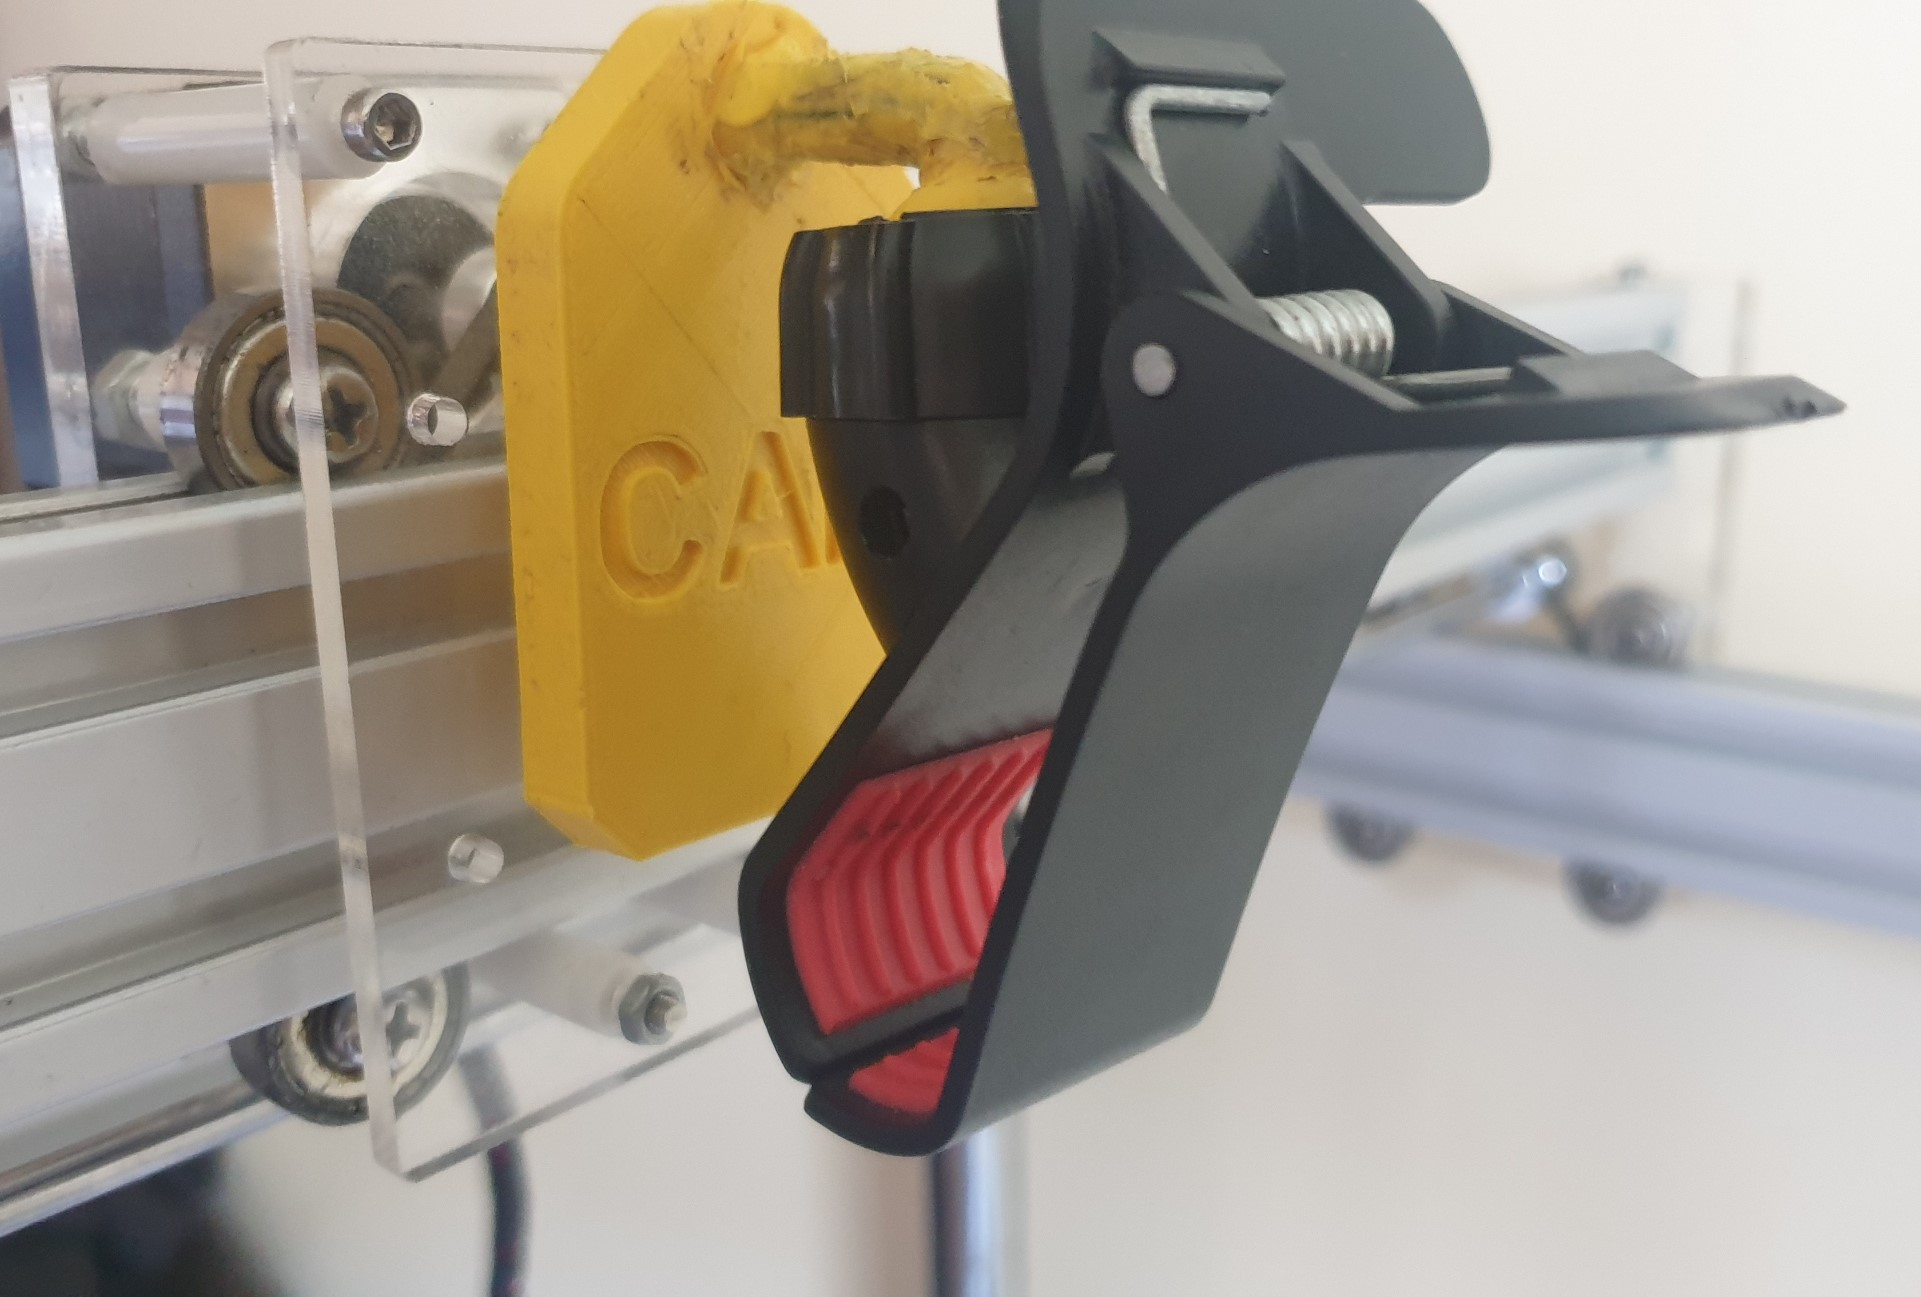
\includegraphics[height=4.5cm]{pages/dodatekARobot/img/mocowanieUchwytu.jpg}
	\end{subfigure}
	\caption{Mocowanie kamery do karetki}
\end{figure}
Do zamocowania telefonu wykorzystany został zacisk uchwytu samochodowego.
Uchwyt mocowany jest poprzez nakrętkę zaciskającą się na wydrukowanej na wysięgniku kuli. 
Takie połączenie pozwala na ustawienie kamery pod dowolnym kątem względem filmowanej powierzchni zachowując wysoką sztywność.
\begin{figure}[H]
	\centering
	\begin{subfigure}{}
		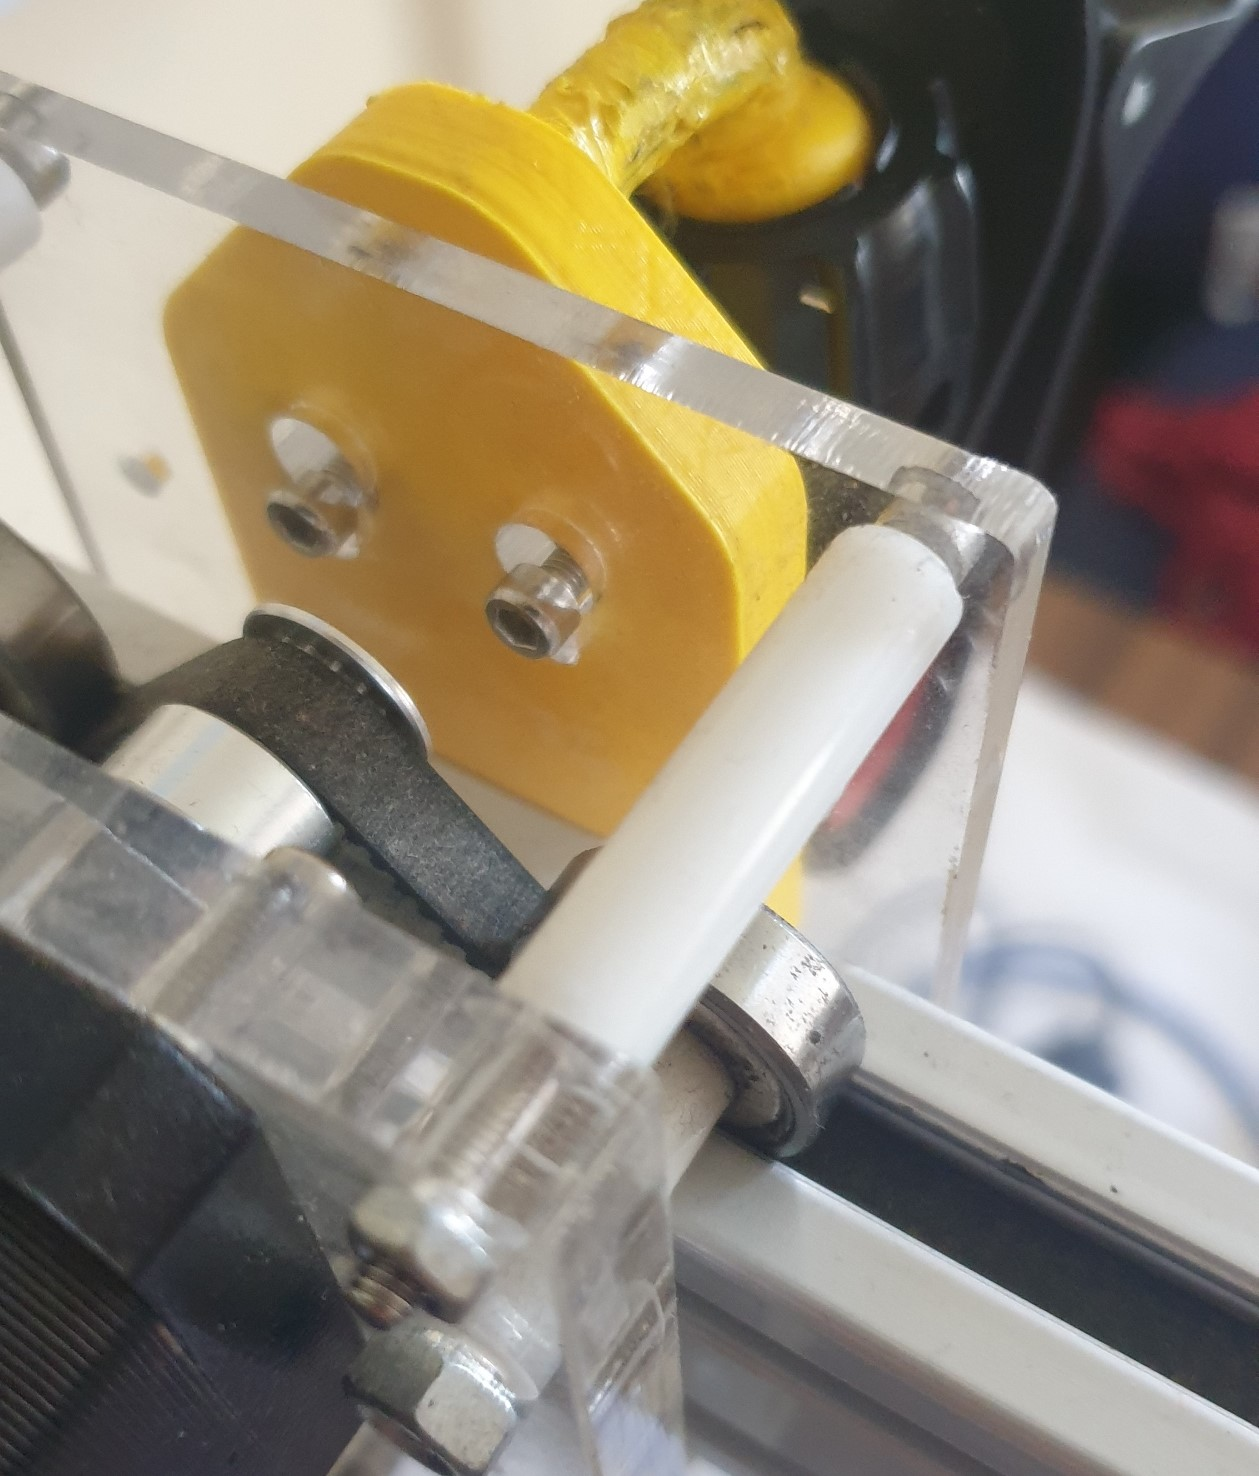
\includegraphics[height=5cm]{pages/dodatekARobot/img/mocownanieUchwytKaretka.jpg}
	\end{subfigure}
	\begin{subfigure}{}
		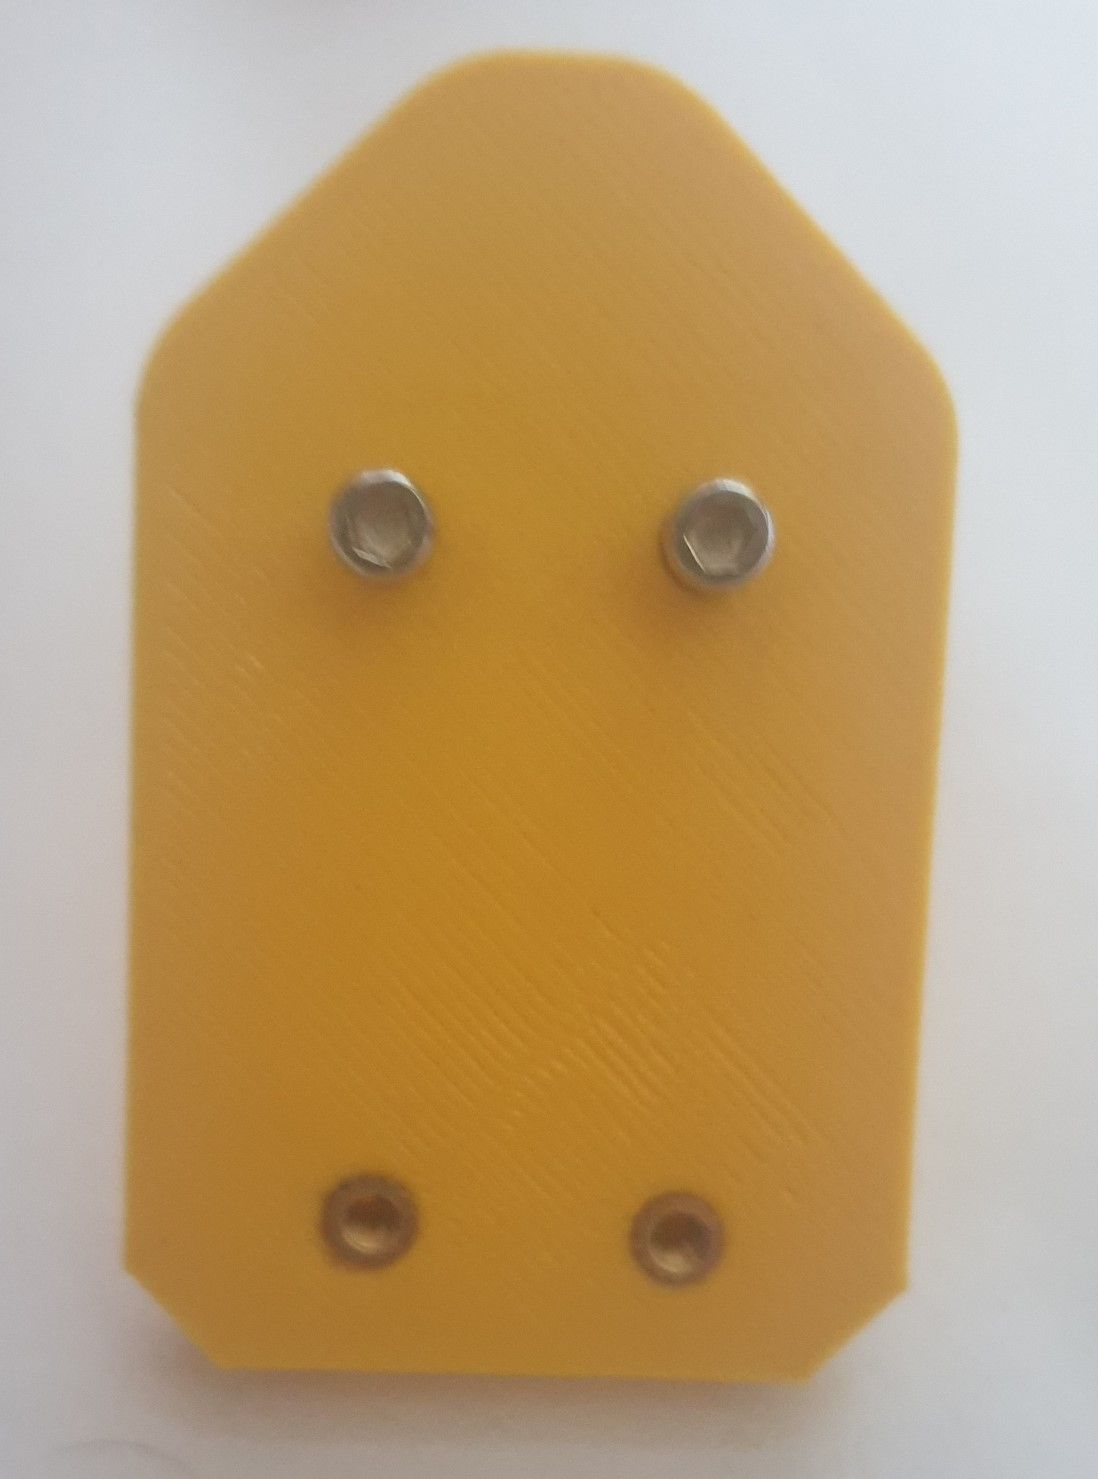
\includegraphics[height=5cm]{pages/dodatekARobot/img/mocowanieKameryTyl.jpg}
	\end{subfigure}
	\caption{Połączone mocowanie i karetka robota}
\end{figure}
Do przygotowanych otworów zostały na gorąco wciśnięte mosiężne, gwintowane tulejki, które pozwalają na wkręcenie śrub z gwintem M3.
Dzięki nim uchwyt może być sztywnie zamocowany.
Finalnie okazało się, że do sztywnego połączenia tych dwóch powierzchni wystarczą tylko dwie śruby.

\textbf{Napędy} \newline
Do napędzania obu osi robota wykorzystane zostały dwa silniki krokowe 4240-15A, o maksymalnym prądzie 1A, kroku osi 1.8$^\circ$ i maksymalnym momencie 53Ncm.
Silniki przykręcone są do grubej płyty typu 'plexa'.
\begin{figure}[H]
	\centering
	\begin{subfigure}{}
		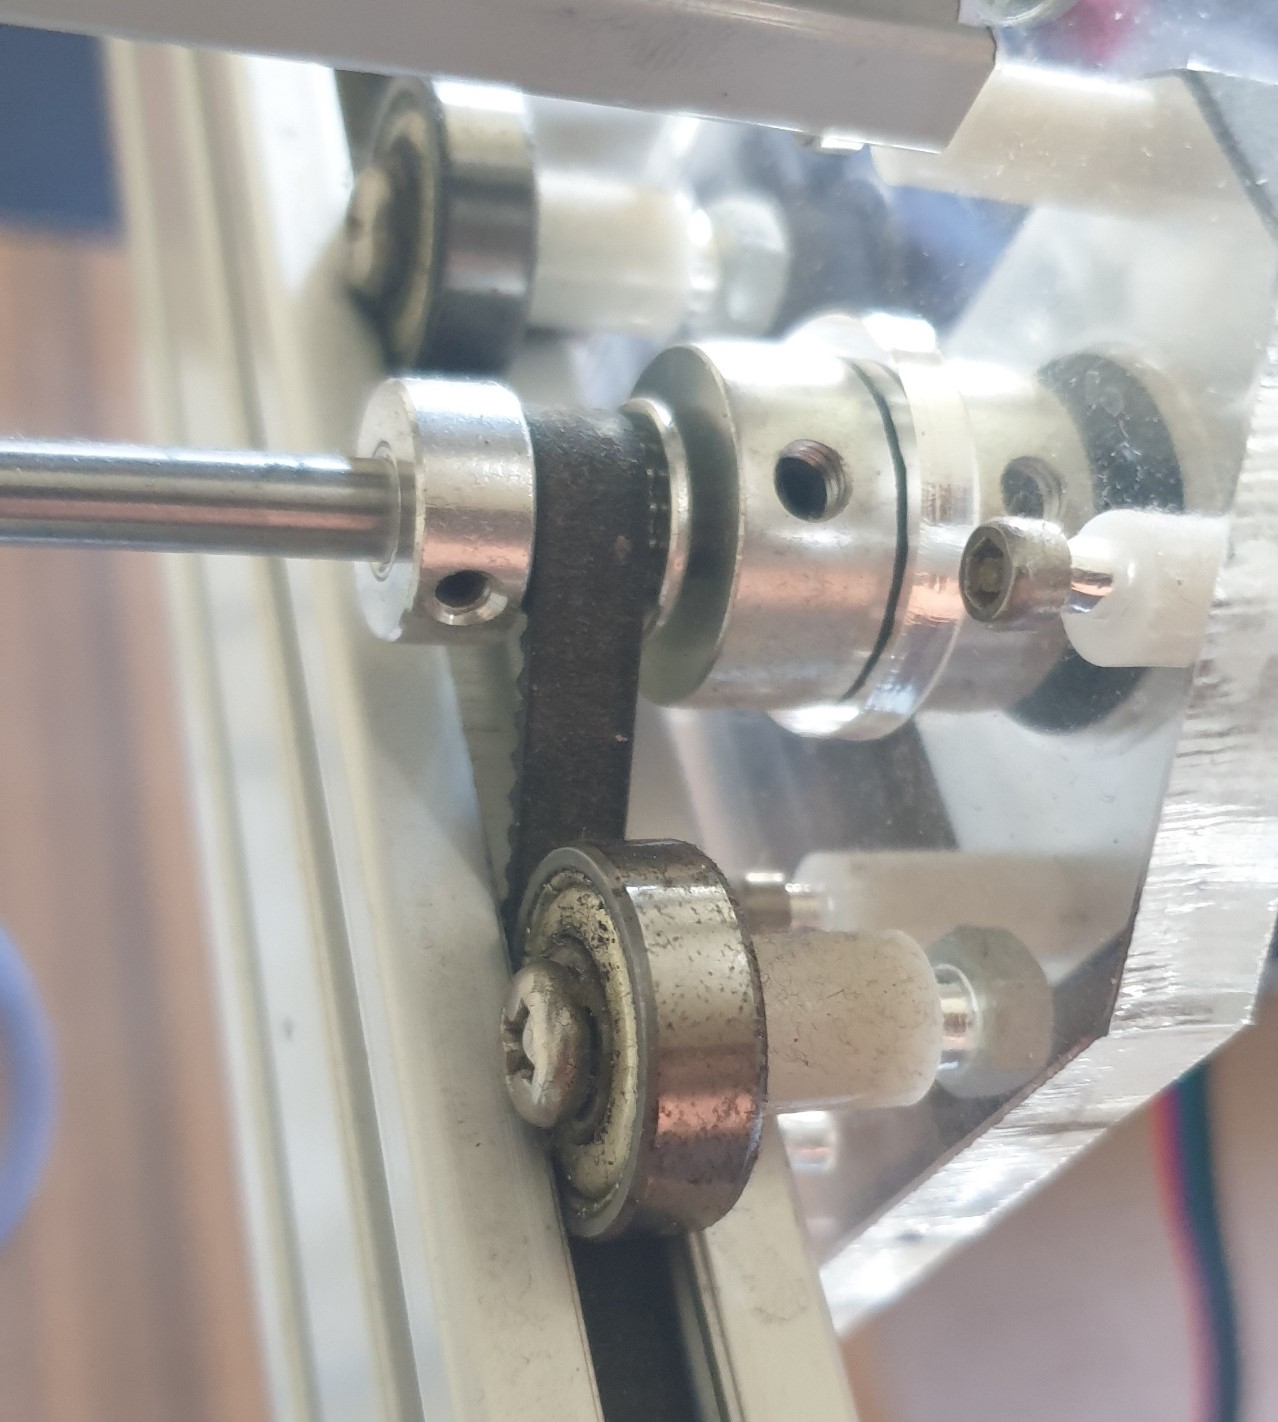
\includegraphics[height=5cm]{pages/dodatekARobot/img/przeniesienieNapedu.jpg}
	\end{subfigure}
	\begin{subfigure}{}
		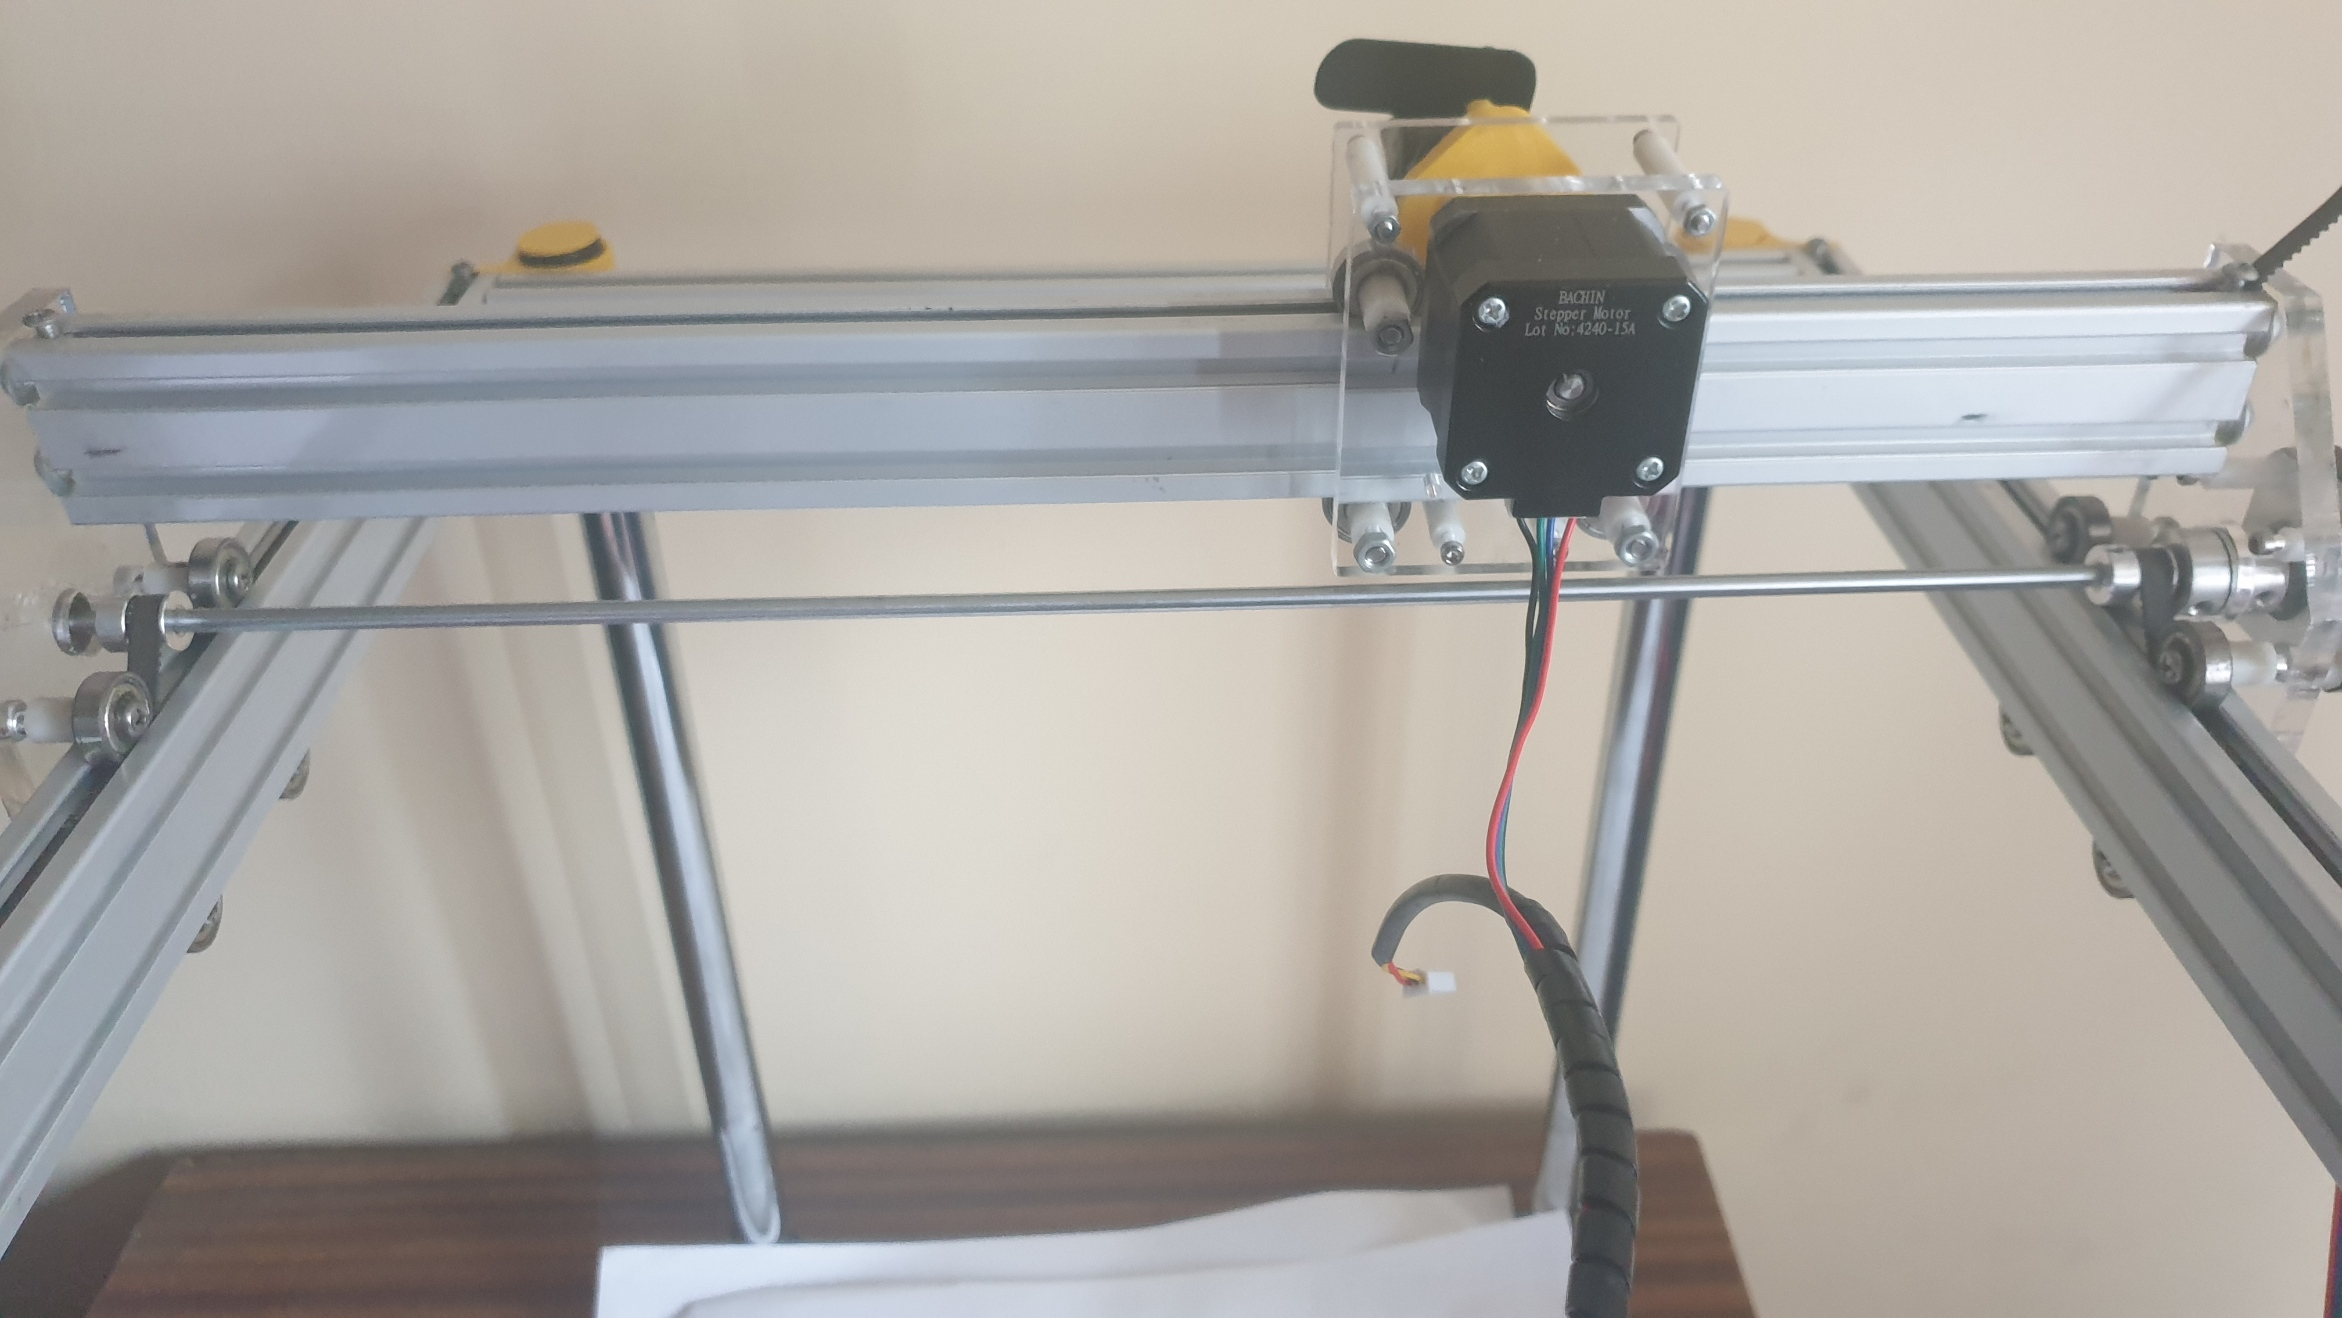
\includegraphics[height=5cm]{pages/dodatekARobot/img/ramaNapedCaly.jpg}
	\end{subfigure}
	\caption{Przekazanie napędu dla pierwszej osi}
\end{figure}
Pierwsze zdjęcie z lewej pokazuje napęd osi, po której porusza się karetka z zamocowanym kolejnym napędem. Widać że na osi silnika 
zamocowane jest sprzęgło podatne (kompensujące drgania), które połączone jest z wałkiem napędowym. 
Na obu końcach wałka zamocowane są koła zębate napędzające pasek GT-2. Pasek przymocowany jest na sztywno do ramy a naciąg kontrolowany jest przez
dwa dociskające go łożyska. Przeniesienie napędu na drugą stronę, konieczne jest ze względu na dosyć dużą ramę i możliwe skrzywianie się podczas ruchu.
\begin{figure}[H]
	\centering
	\begin{subfigure}{}
		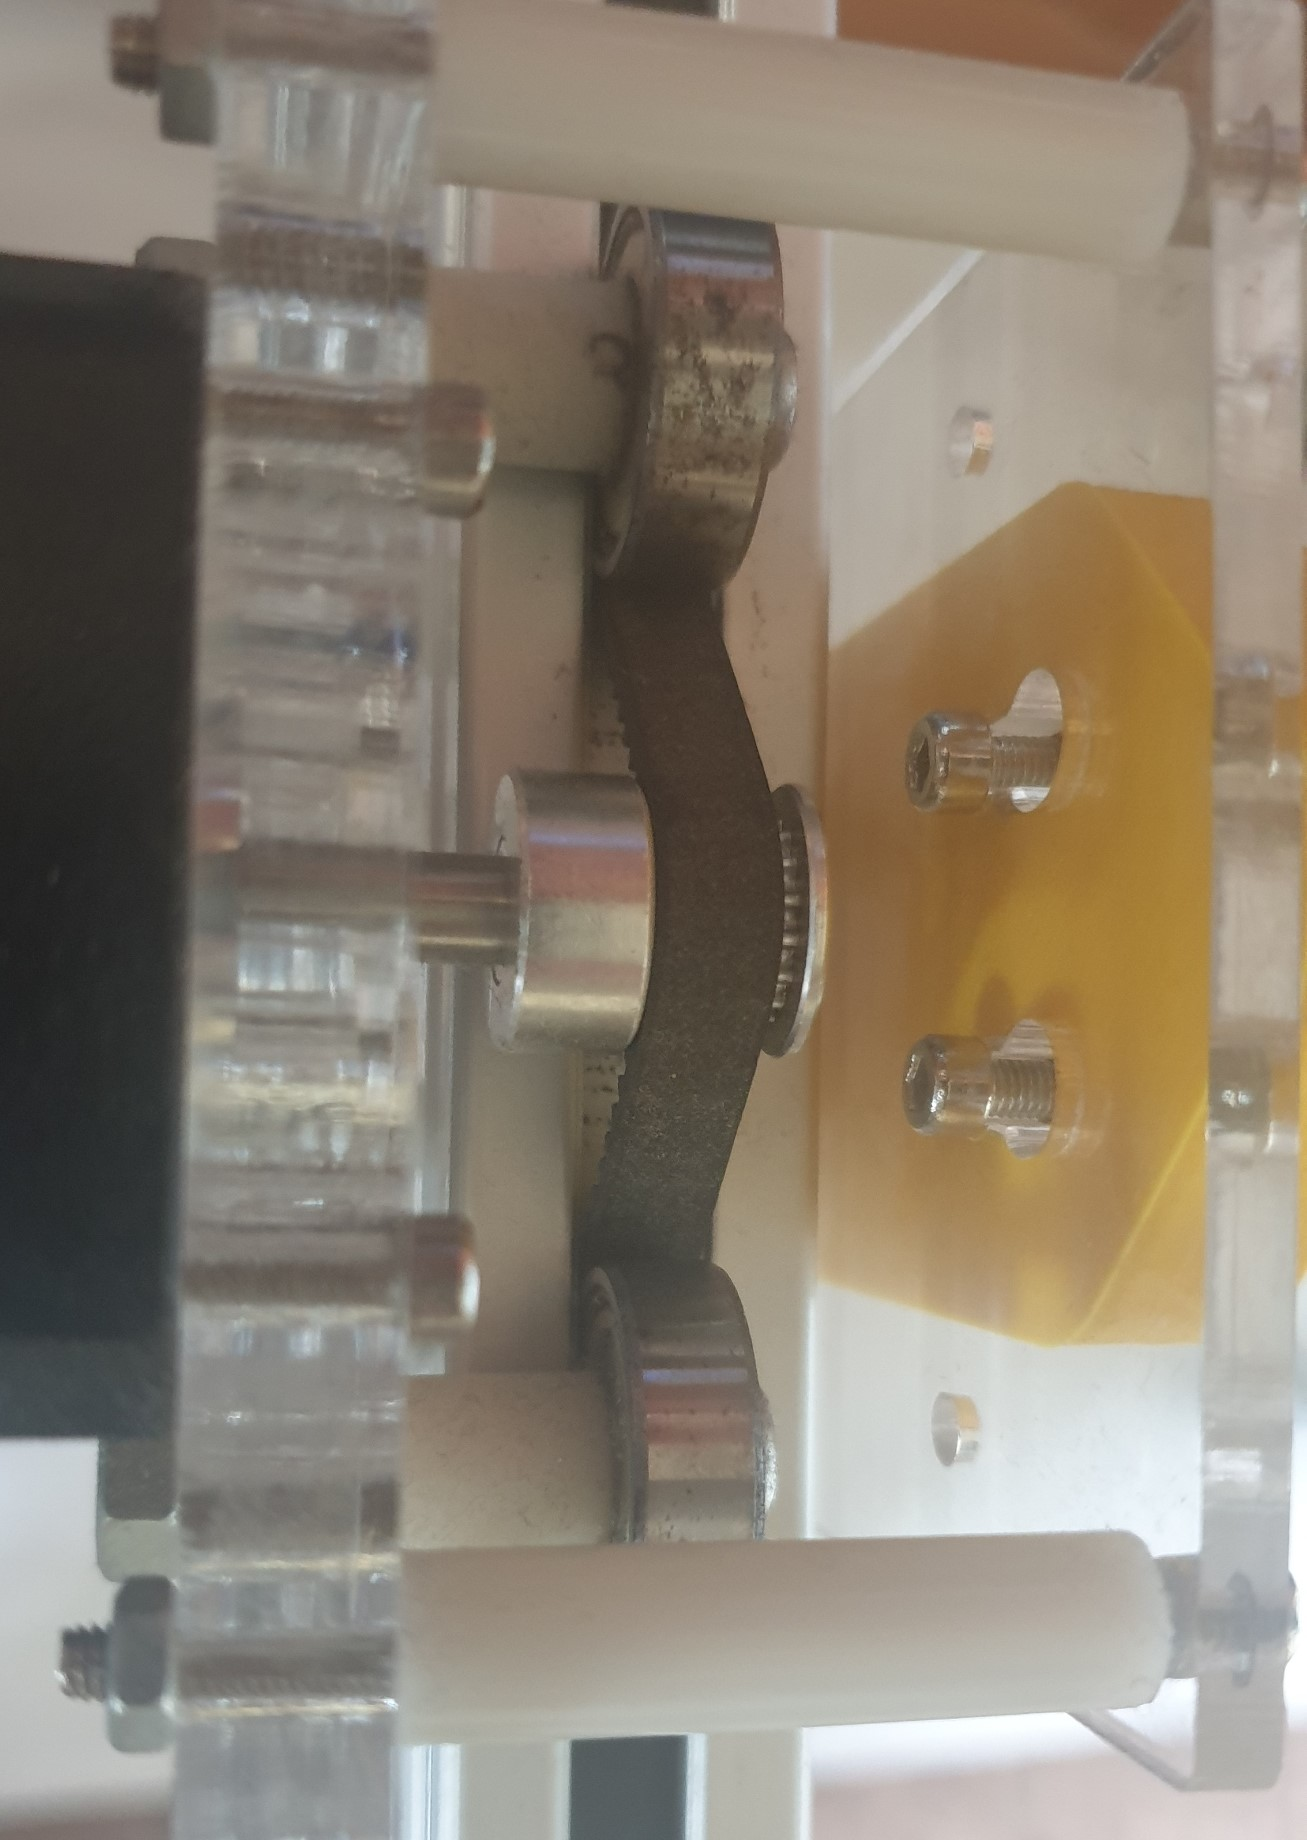
\includegraphics[height=5.5cm]{pages/dodatekARobot/img/przeniesienieNapeduW2.jpg}
	\end{subfigure}
	\begin{subfigure}{}
		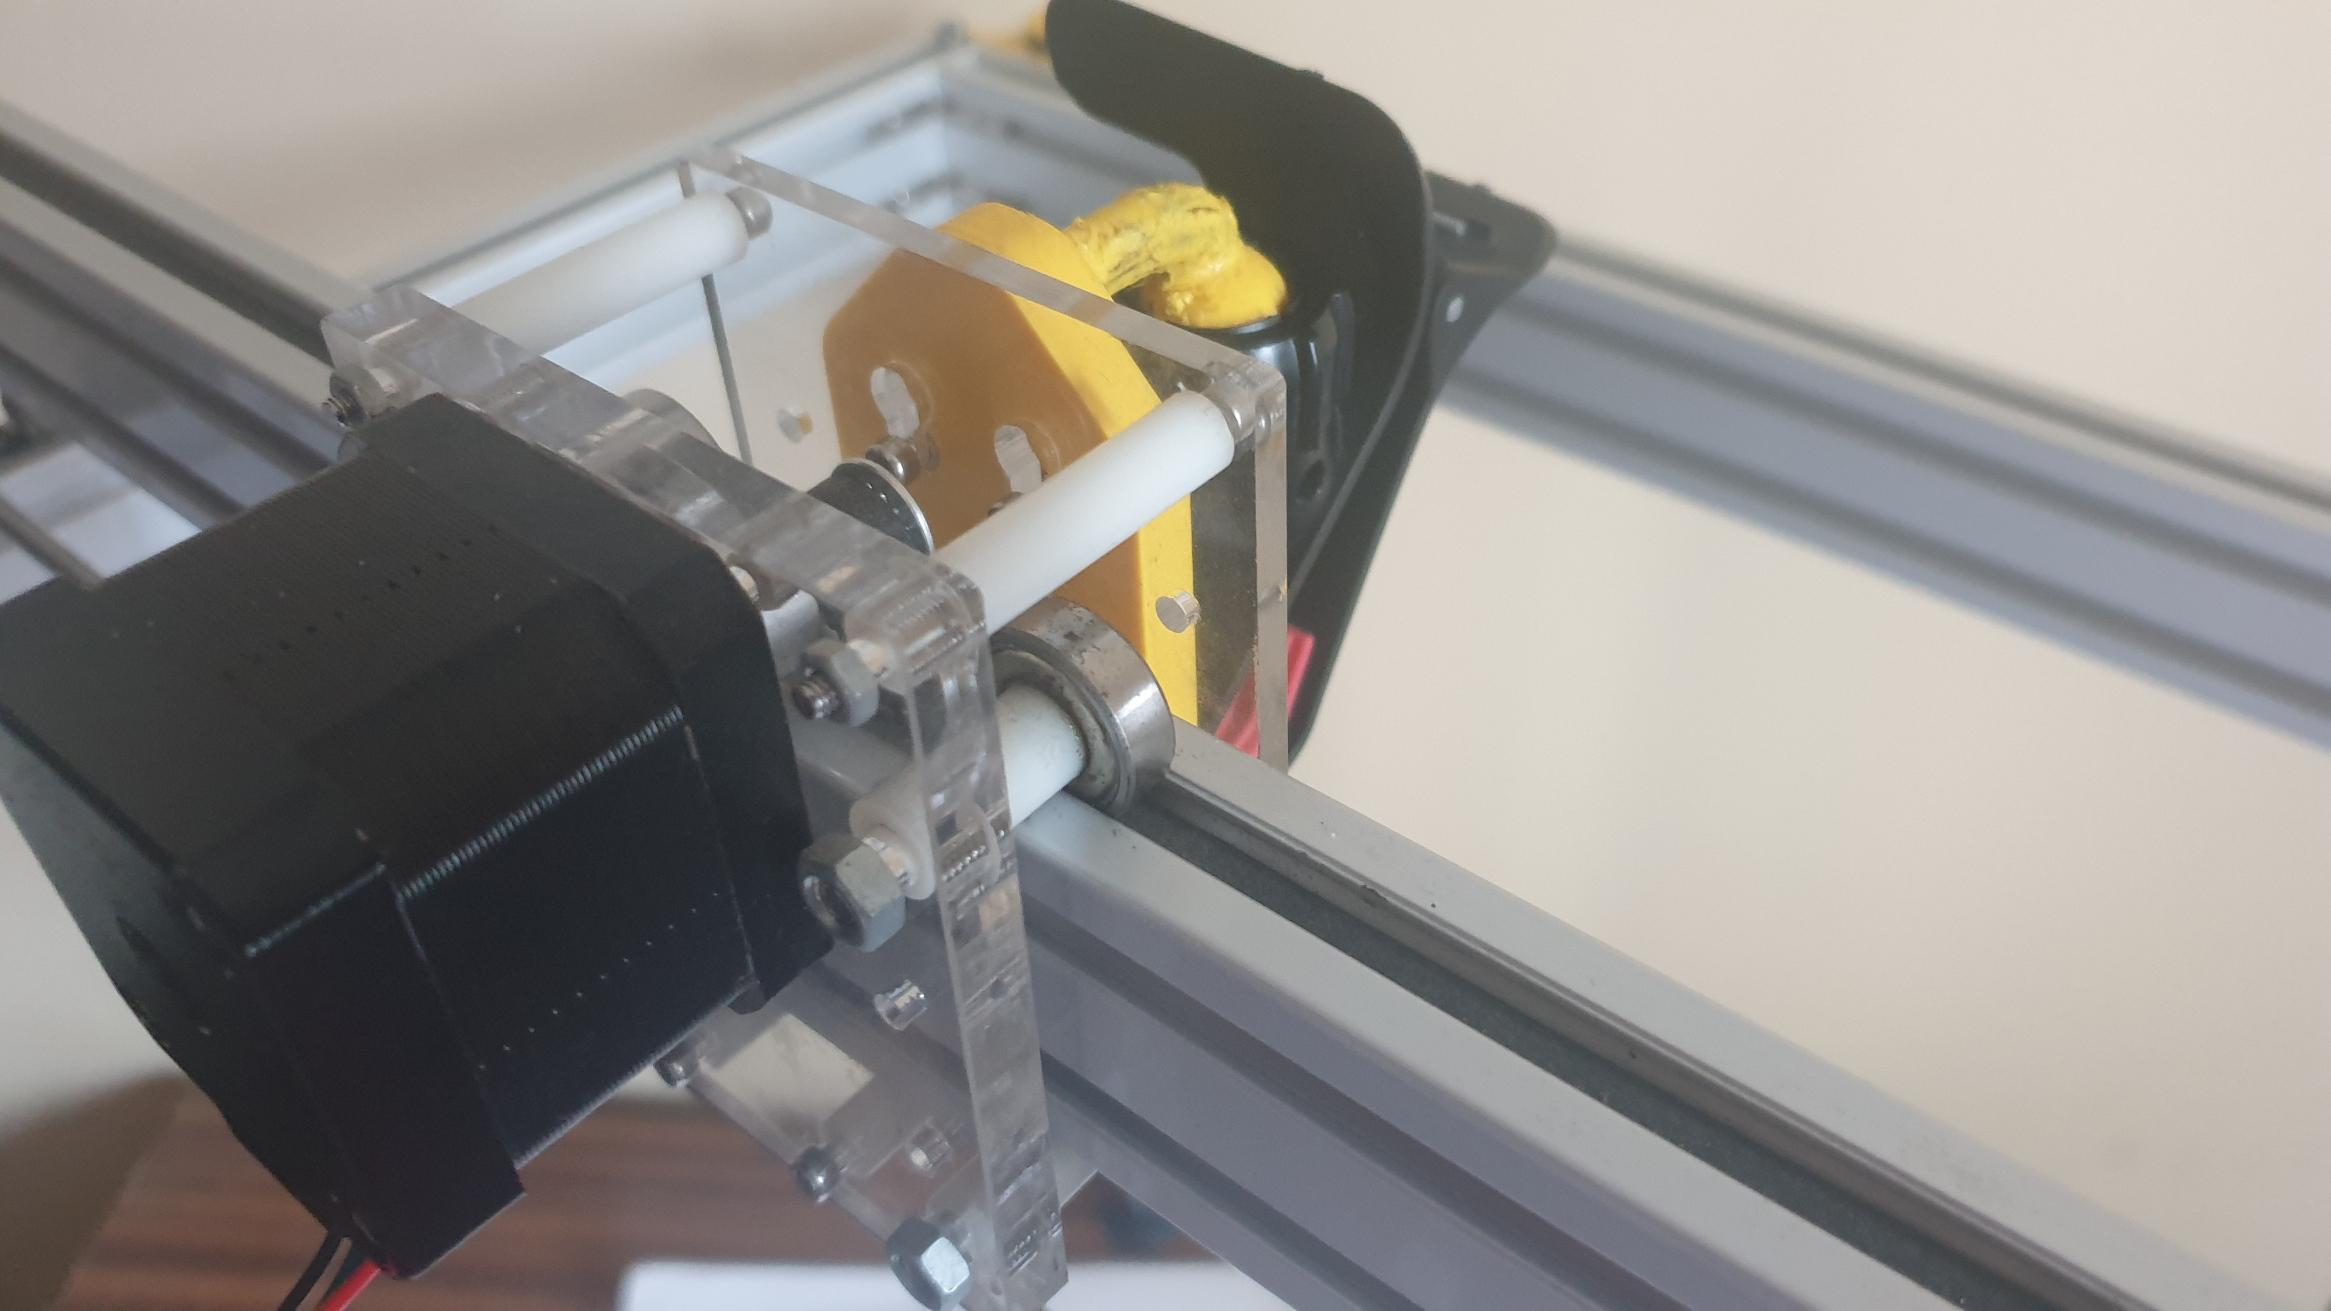
\includegraphics[height=5.5cm]{pages/dodatekARobot/img/widokNaOs2.jpg}
	\end{subfigure}
	\caption{Napęd osi przesuwającą karetką}
\end{figure}
Napęd drugiej osi został zrealizowany identycznie, poza tym że w tym przypadku koło zębate jest zamocowane bezpośrednio na osi silnika.

\textbf{Sterowanie i komunikacja} \newline
Sterowanie zrealizowane jest przy pomocy mikrokontrolera Arduino Nano i płytki z odpowiednimi sterownikami silników krokowych. 
Sterownik ma wgrany program pozwalający, na komunikacje z komputerem przy pomocy portu szeregowego i analizę wysyłanych komend G-Code.
Komendy pozwalają na poruszanie robotem z określoną prędkością lub modyfikacje parametrów pracy np. przejście z współrzędnych absolutnych na przyrostowe.

\begin{figure}[H]
	\centering
	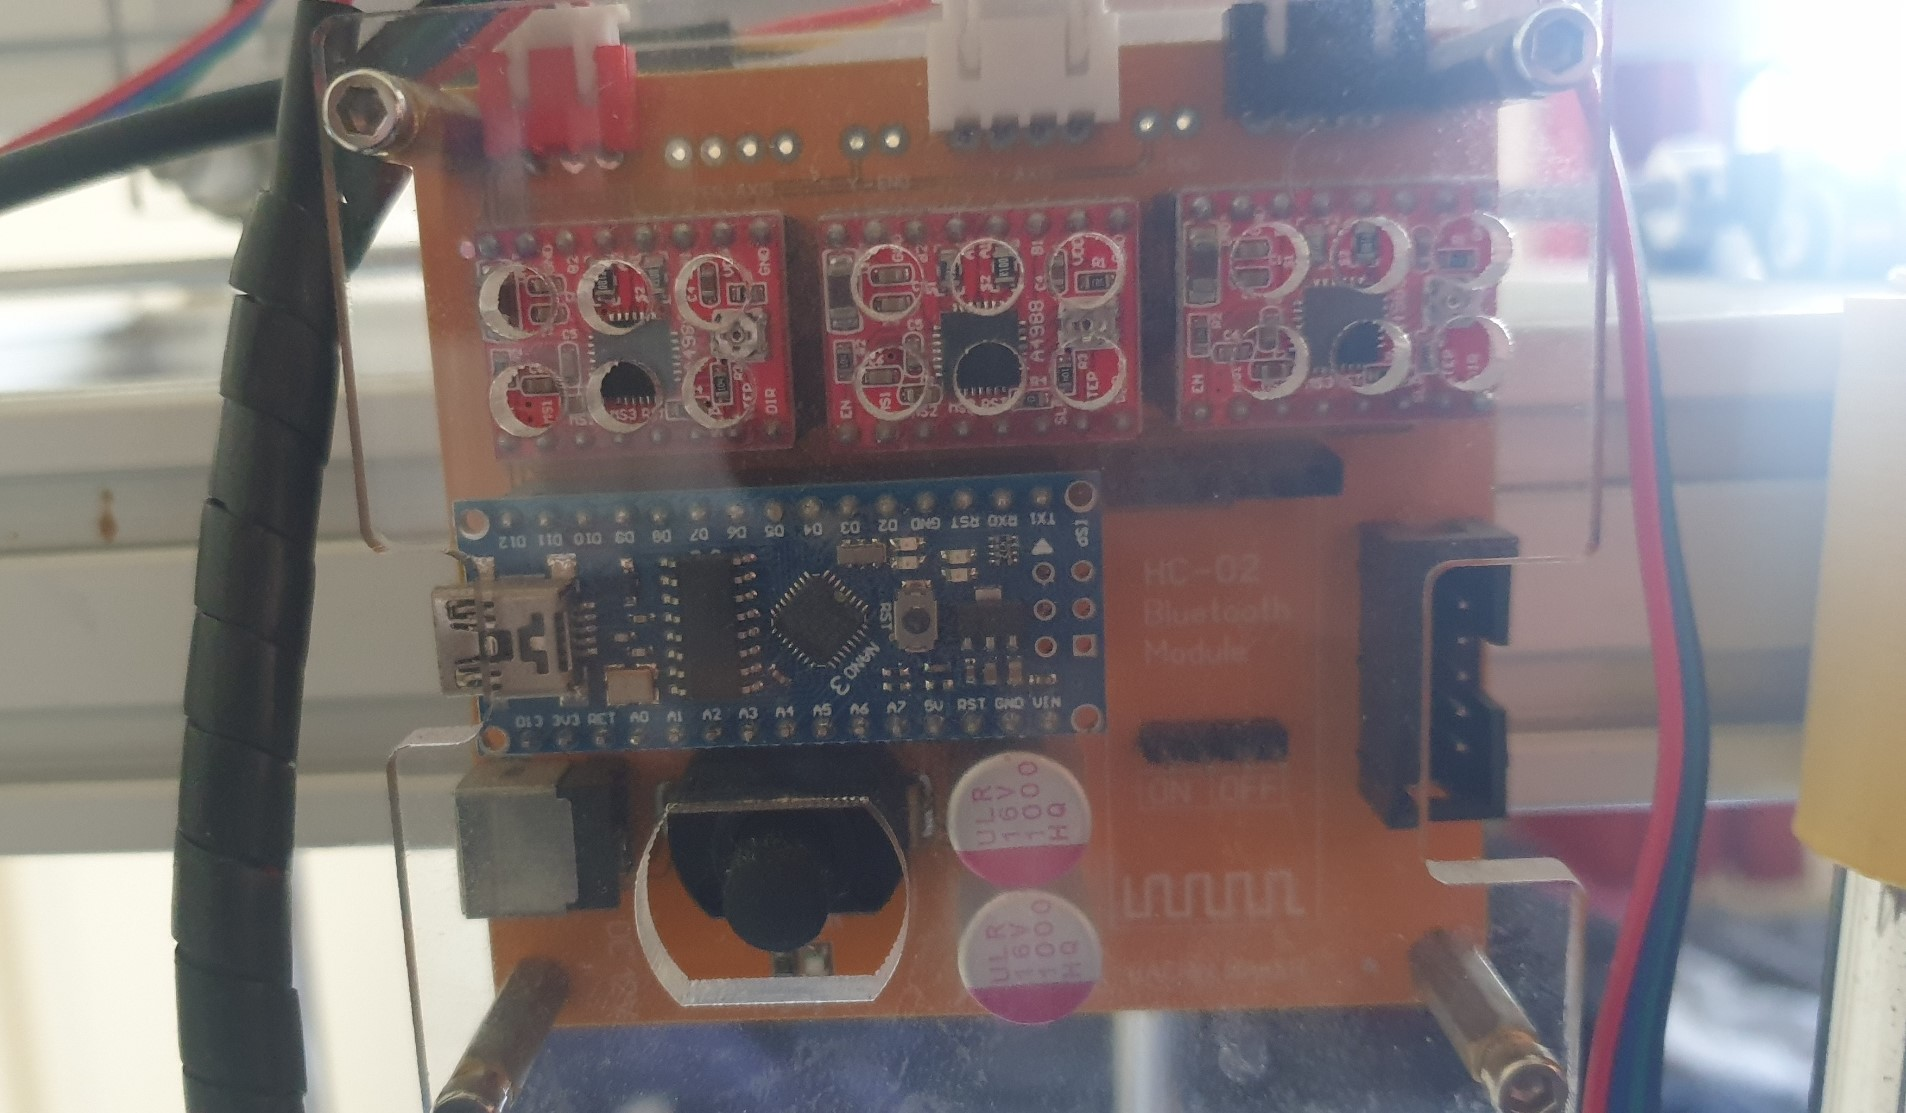
\includegraphics[width=0.70\linewidth]{pages/dodatekARobot/img/kontroler.jpg}
	\caption{Zdjęcie sterownika}
\end{figure}
Wykorzystano sterowniki silników krokowych opartych na układzie A4988. 
Modułowe sterowniki, pozwalają na szybką wymianę w przypadku awarii.

\textbf{Oprogramowanie sterownika} \newline
Do sterowania silnikami i interpretacji wysyłanych poleceń w formacie G-Code użyto otwartego projektu 
grbl\cite{grblGithub} w wersji 1.1f. Repozytorium z całym projektem można pobrać ze strony github. 
Dzięki zastosowaniu otwartego projektu, sterownik od razu zna wszystkie potrzebne komendy takie jak 
G0 (szybki ruch liniowy), G1 (ruch liniowy z narzędziem) czy inne jak G53 (zmiana systemu współrzędnych na absolutne).
Do uruchomienia projektu, potrzebujemy program Arduino IDE, które zawiera w sobie kompilator i potrzebny program programujący 
mikrokontroler sterownika. Przed kompilacją należy wskazać konkretne piny odpowiadające za sterowanie silnikami. 
Po wgraniu programu należy odpowiednio skonfigurować podstawowe parametry np. ilość kroków silnika potrzebną do przesunięcia się o 1mm. 
Ustawienia i zapisania parametrów dokonuje się poprzez wysłanie odpowiedniej kombinacji poleceń przy pomocy dowolnego 
terminala łączącego się poprzez port szeregowy np. PuTTy.

\textbf{Kamera} \newline
W tym przypadku jako kamerę wykorzystano telefon z zainstalowaną aplikacją iVCam. Aby połączyć się z komputera należy zainstalować 
program kliencki iVCam, który dodaje wirtualną kamerę do systemu. 
\begin{figure}[H]
	\begin{subfigure}{}
		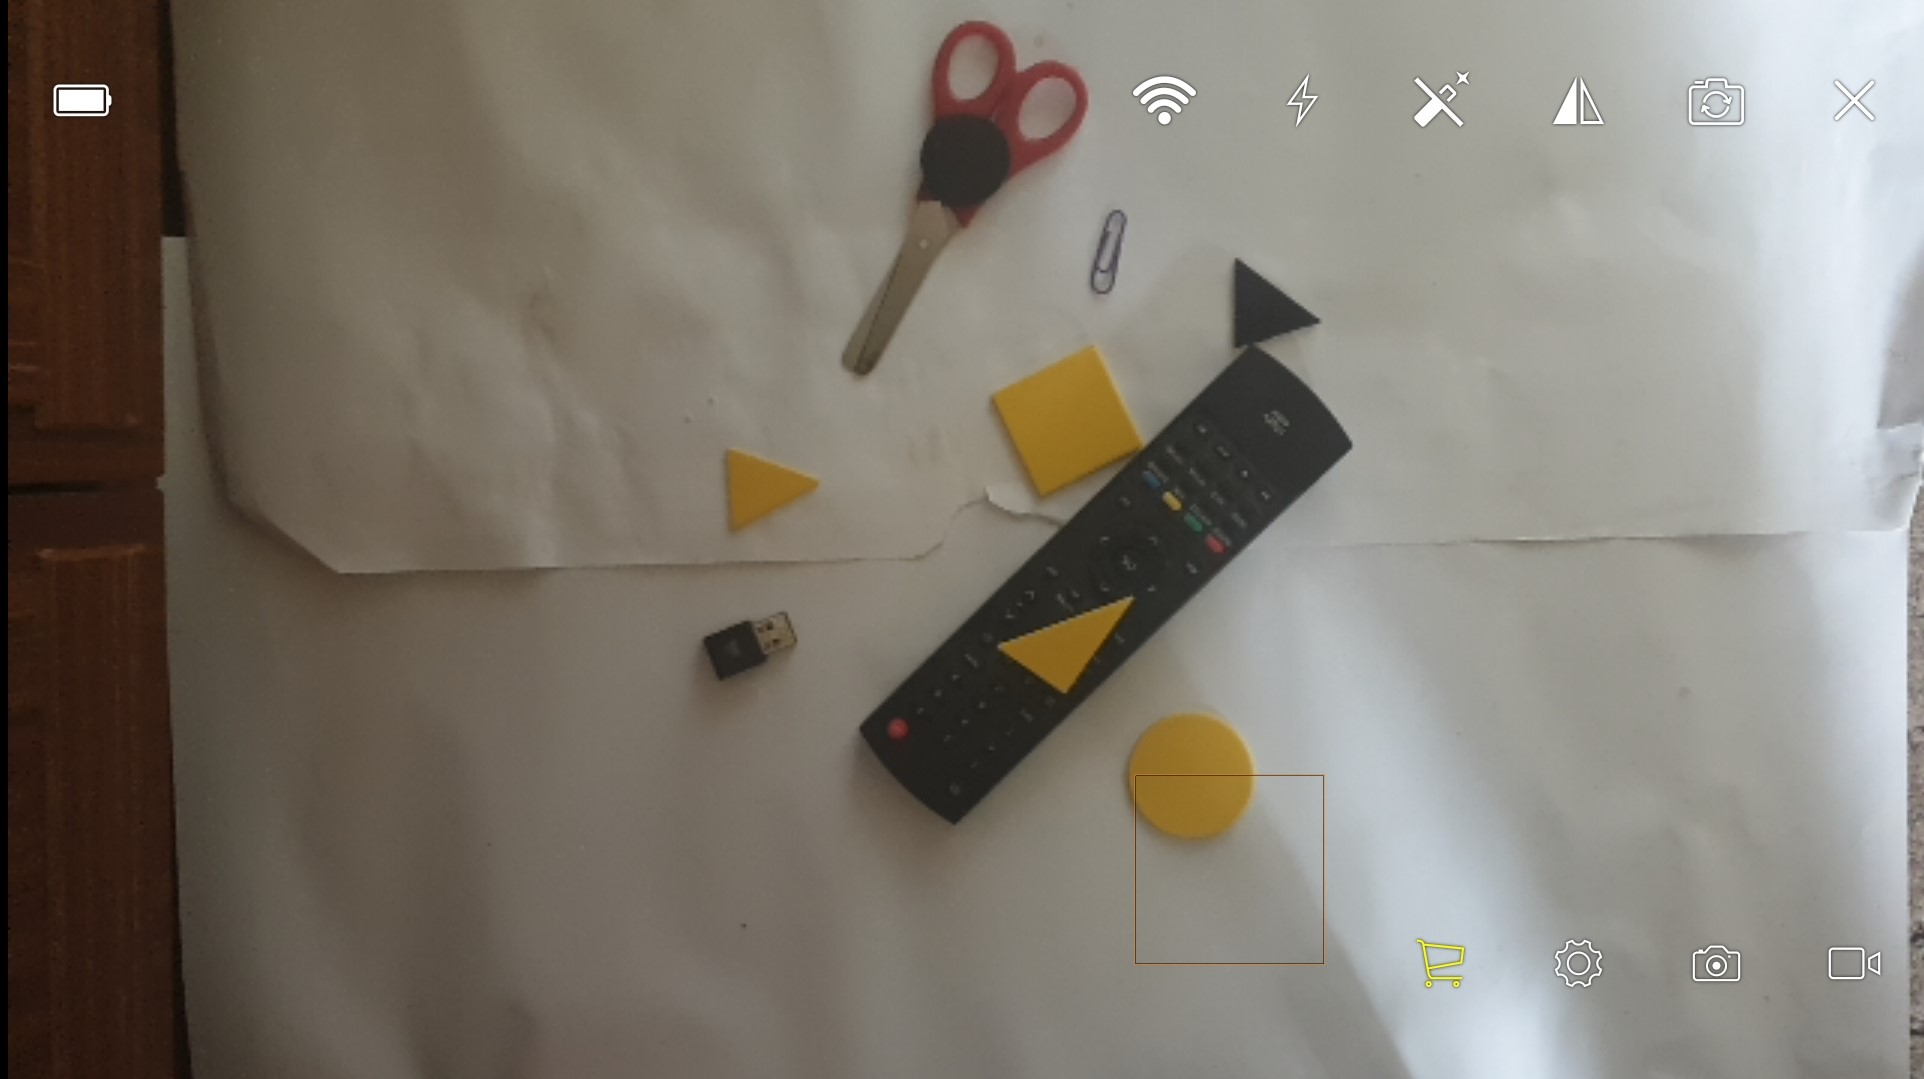
\includegraphics[height=4.5cm]{pages/dodatekARobot/img/kameraTelefon.jpg}
	\end{subfigure}
	\begin{subfigure}{}
		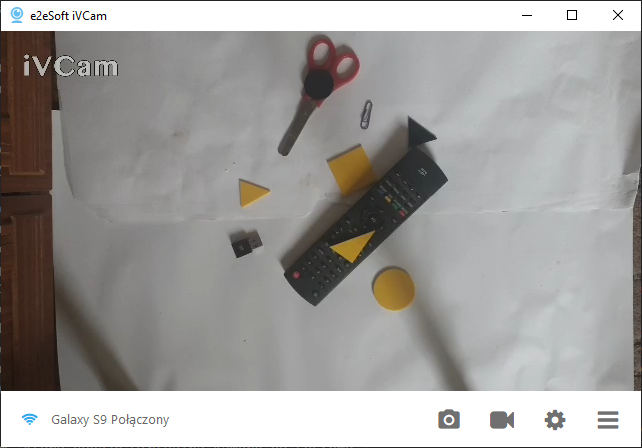
\includegraphics[height=4.5cm]{pages/dodatekARobot/img/kameraDesktop.png}
	\end{subfigure}
	\caption{Połączenie telefonu i komputera przy pomocy aplikacji iVCam}
\end{figure}

Jak widać na powyższym zdjęciu, telefon połączył się z aplikacją zainstalowana na komputerze. 
Aplikacja imituje zwykłą kamerę widoczną przez system operacyjny, dzięki czemu nie była potrzebna żadna dodatkowa 
biblioteka do obsługi połączenia bezprzewodowego. 
W porównaniu do wcześniej testowanym protokołem RTSP, to rozwiązanie cechuje się bardzo niskim opóźnieniem i dobrą jakością 
przesyłanego obrazu. Wadą aplikacji jest znak wodny z logiem, jednak nie przeszkadzał on w pracy sieci neuronowej. 